\section{Sumber Data}
Penelitian ini dilakukan menggunakan data sekunder secara daring tanpa melakukan pengambilan data di lapangan. Seluruh proses analisis dan pengolahan data dilakuakn secara komputasi di lingkugan pengolahan data statistik. Penelitian ini berlangsung dalam rentang waktu Januari hingga Juni 2025. 

Data utama yang digunakan dalam penelitian ini adalah data curah hujan harian berbasis satelit yang diperoleh dari NASA \textit{(National Aeronnautics and Space Administration)} melalui platform \textit{ POWER Data Access Viewer}. Data ini mencakup informasi spasial (koordinat grid wilayah) dan temporal (periode waktu pengamatan) yang diperlukan dalam pemodelan spasio temporal menggunakan STARMA. 

Selain itu, informasi koordinat geografis yang merepresentasikan lokasi grid atau titik observasi juga digunakan untuk membangun \textit{spatial weight matrix} yang merepresentasikam kedekatakan spasial antar wilayah. Data pendukung ini diambil langusng dari metadata bawaan dataset NASA yang digunakan. 
Berikut merupakan gambar sumber data yang digunakan dalam penelitian ini:
\begin{figure}[H]
    \centering
    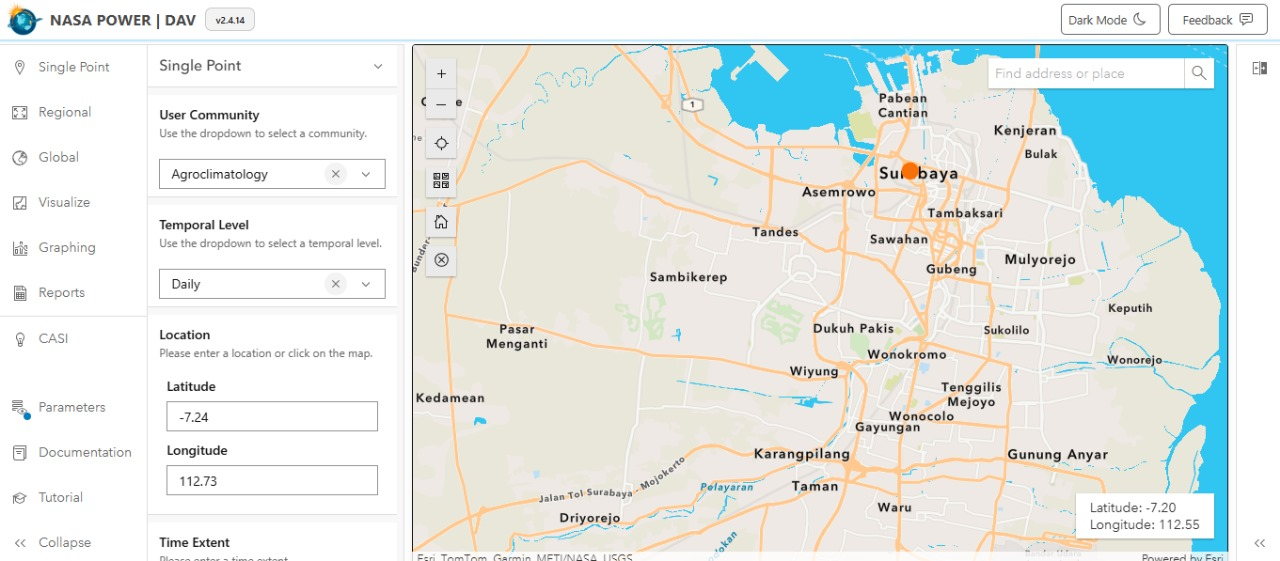
\includegraphics[width=0.9\textwidth]{images/bab_3/nasa.jpg}
    \caption{Data NASA Wilayah Surabaya}
    \label{fig:flowchart-pemodelan}
\end{figure}

\subsection{Data Sekunder}
\begin{longtable}{|l|c|c|c|c|}
    \caption{Data Curah Hujan Bulanan Berdasarkan Wilayah}
    \label{table:data_sekunder} \\
    \hline
    \textbf{Wilayah} & \textbf{Latitude} & \textbf{Longitude} & \textbf{Date} & \textbf{Precipitation} \\
    \hline
    \endfirsthead

    \hline
    \textbf{Wilayah} & \textbf{Latitude} & \textbf{Longitude} & \textbf{Date} & \textbf{Precipitation} \\
    \hline
    \endhead

    \hline
    \endfoot

    \hline
    \endlastfoot

    % ================= UTARA =================
    Utara  & -7.2 & 112.73 & 1/31/2015 & 13.89 \\
    Utara  & -7.2 & 112.73 & 2/28/2015 & 11.93 \\
    Utara  & -7.2 & 112.73 & 3/31/2015 & 9.38 \\
    \multicolumn{1}{|c|}{\raisebox{0.5ex}{$\vdots$}} &
    \multicolumn{1}{c|}{\raisebox{0.5ex}{$\vdots$}} &
    \multicolumn{1}{c|}{\raisebox{0.5ex}{$\vdots$}} &
    \multicolumn{1}{c|}{\raisebox{0.5ex}{$\vdots$}} &
    \multicolumn{1}{c|}{\raisebox{0.5ex}{$\vdots$}} \\  
    Utara  & -7.2 & 112.73 & 10/31/2024 & 1.12 \\
    Utara  & -7.2 & 112.73 & 11/30/2024 & 6.53 \\
    Utara  & -7.2 & 112.73 & 12/31/2024 & 13.60 \\
    \hline

    % ================= BARAT =================
    Barat  & -7.24 & 112.61 & 1/31/2015 & 13.92 \\
    Barat  & -7.24 & 112.61 & 2/28/2015 & 11.87 \\
    Barat  & -7.24 & 112.61 & 3/31/2015 & 9.44 \\
    \multicolumn{1}{|c|}{\raisebox{0.5ex}{$\vdots$}} &
    \multicolumn{1}{c|}{\raisebox{0.5ex}{$\vdots$}} &
    \multicolumn{1}{c|}{\raisebox{0.5ex}{$\vdots$}} &
    \multicolumn{1}{c|}{\raisebox{0.5ex}{$\vdots$}} &
    \multicolumn{1}{c|}{\raisebox{0.5ex}{$\vdots$}} \\  
    Barat  & -7.24 & 112.61 & 10/31/2024 & 1.46 \\
    Barat  & -7.24 & 112.61 & 11/30/2024 & 6.29 \\
    Barat  & -7.24 & 112.61 & 12/31/2024 & 13.62 \\
    \hline

    % ================= TIMUR =================
    Timur  & -7.31 & 112.84 & 1/31/2015 & 12.24 \\
    Timur  & -7.31 & 112.84 & 2/28/2015 & 10.29 \\
    Timur  & -7.31 & 112.84 & 3/31/2015 & 8.84 \\
    \multicolumn{1}{|c|}{\raisebox{0.5ex}{$\vdots$}} &
    \multicolumn{1}{c|}{\raisebox{0.5ex}{$\vdots$}} &
    \multicolumn{1}{c|}{\raisebox{0.5ex}{$\vdots$}} &
    \multicolumn{1}{c|}{\raisebox{0.5ex}{$\vdots$}} &
    \multicolumn{1}{c|}{\raisebox{0.5ex}{$\vdots$}} \\  
    Timur  & -7.31 & 112.84 & 10/31/2024 & 1.22 \\
    Timur  & -7.31 & 112.84 & 11/30/2024 & 5.63 \\
    Timur  & -7.31 & 112.84 & 12/31/2024 & 12.31 \\
    \hline

    % ================= SELATAN =================
    Selatan & -7.35 & 112.73 & 1/31/2015 & 14.30 \\
    Selatan & -7.35 & 112.73 & 2/28/2015 & 12.15 \\
    Selatan & -7.35 & 112.73 & 3/31/2015 & 11.21 \\
    \multicolumn{1}{|c|}{\raisebox{0.5ex}{$\vdots$}} &
    \multicolumn{1}{c|}{\raisebox{0.5ex}{$\vdots$}} &
    \multicolumn{1}{c|}{\raisebox{0.5ex}{$\vdots$}} &
    \multicolumn{1}{c|}{\raisebox{0.5ex}{$\vdots$}} &
    \multicolumn{1}{c|}{\raisebox{0.5ex}{$\vdots$}} \\  
    Selatan & -7.35 & 112.73 & 10/31/2024 & 1.24 \\
    Selatan & -7.35 & 112.73 & 11/30/2024 & 6.63 \\
    Selatan & -7.35 & 112.73 & 12/31/2024 & 13.51 \\
    \hline

    % ================= TENGAH =================
    Tengah & -7.26 & 112.74 & 1/31/2015 & 14.25 \\
    Tengah & -7.26 & 112.74 & 2/28/2015 & 12.17 \\
    Tengah & -7.26 & 112.74 & 3/31/2015 & 11.19 \\
    \multicolumn{1}{|c|}{\raisebox{0.5ex}{$\vdots$}} &
    \multicolumn{1}{c|}{\raisebox{0.5ex}{$\vdots$}} &
    \multicolumn{1}{c|}{\raisebox{0.5ex}{$\vdots$}} &
    \multicolumn{1}{c|}{\raisebox{0.5ex}{$\vdots$}} &
    \multicolumn{1}{c|}{\raisebox{0.5ex}{$\vdots$}} \\  
    Tengah & -7.26 & 112.74 & 10/31/2024 & 0.83 \\
    Tengah & -7.26 & 112.74 & 11/30/2024 & 6.66 \\
    Tengah & -7.26 & 112.74 & 12/31/2024 & 13.59 \\
    \hline

\end{longtable}